\documentclass[12pt]{article}
\usepackage{amsmath, amsthm, amssymb, enumerate, mathrsfs, graphicx, subfig, verbatim, float, pdflscape, rotating, parskip, setspace, tikz, tikz-qtree, url, epstopdf, mathtools, latexsym, flexisym,accents, multirow,diagbox,accents}
\usepackage[framed,numbered,autolinebreaks,useliterate]{mcode}
\usepackage{url}
\usepackage{listings}
\usepackage{pdfpages}
\usepackage{breqn}

\usepackage[margin=1in]{geometry}
\usepackage[round]{natbib}
\addtolength{\parskip}{\baselineskip}
\DeclareMathSizes{12}{13}{7}{7}
\usepackage[bottom]{footmisc}
\newcommand{\ubar}[1]{\underaccent{\bar}{#1}}

\parskip 2pt
\setlength\parindent{0cm}
\begin{document}
\begin{onehalfspace}


\title{Econ 8307\\ Assignment 2 (Spring 2019)}
\author{Jonah Coste, Fred Xu\\George Washington University}
\date{}
\maketitle
\parskip 10pt
\textbf{Question 1}\\

\begin{lstlisting}
beta = .97;
delta = .1;
theta = .3;
steady=@(x) [-x(1) + beta*x(1)*(theta * x(2)^(theta-1) + 1 - delta);
	x(2)^theta - delta*x(2) - x(1)];

initial_guess=[1;1];


steady_state=fsolve(steady,initial_guess)
\end{lstlisting}
Prints the steady state solution. Thew first entry is steady state consumption and the second entry is steady state capital.
\begin{lstlisting}
steady_state =

    1.0998
    3.2690
\end{lstlisting}


\textbf{Question 2}\\
\begin{enumerate}[1.]
	\item
Define E as a row matrix with two variables. Each variable is an indicator for employed or unemplyed i.e. $E=[1,0]$ if employed and $E=[0,1]$ if unemployed. This is the state variable. Value function becomes Value(E) = EV where V is a 1x2 column vector: $V = [value\ if\ employed ; value\ if\ unemployed]$.\\
$Value(E)= EV = EU + \beta*ETV$\\
 Where T is a transition matrix: $T = [pi_e, 1-pi_e; 1-pi_u, pi_u]$, and U is the column matrix $U=[u(w_h); u(w_l)]$
	\item
	\begin{lstlisting}
 w_h = 1;
 w_l = .9;
 beta = .96;
 pi_e = .95;
 pi_u = .9;
 utility=@(c) log(c);

 T = [pi_e, 1-pi_e; 1-pi_u, pi_u];
 U = [utility(1); utility(.9)];
 I = eye(2);
 
 V=inv(I-beta*T)*U;
 V
	\end{lstlisting}
	Prints value function vector.
	\begin{lstlisting}
	V =

   -0.6871
   -1.2597
	\end{lstlisting}
	
	\item
	\begin{lstlisting}
steady2=@(x) (1-pi_e)*(1-x) + pi_u*x - x;
initial_guess2=.5;
unemployment_rate=fsolve(steady2,initial_guess2)
	\end{lstlisting}
	Prints steady state unemployment rate.
	\begin{lstlisting}
	unemployment_rate =

    0.3333
	\end{lstlisting}
\end{enumerate}

\textbf{Question 3}\\

$n^*(z) = (\frac{w}{z\alpha})^{\frac{1}{\alpha-1}}$\\
 
 Let $S_{it} = [s_{it1}; s_{it2}; ... ; s_{itN}]$ be a Nx1 column vector where $s_{itx}=1$ if $z_{it} = z_x$ and 0 otherwise. Therefore, $S_{it}Z = z_{it}$. S_it is the state variable.\\
 The value function is: $Value(S) = SV = S\pi + \beta(1-\lambda)STV$
 Where T is the NxN transition matrix i.e. $T_{jk} = f(z_{i,t+1} = k | z_{it} = j)$ and $\pi$ is the optimal profit row vector $[\pi_1, \pi_2, ... , \pi_N]$ where $\pi_x = z_xn^*(z_x)^\alpha - wn^*(z_x)$
 
\textbf{Question 4}\\

\begin{enumerate}[1.]
	\item
	\begin{lstlisting}
 N = 5;
 p = .8;
 w = 1;
 alpha = .7;
 beta = .95;
 lambda = .1;
 
 Z = zeros(1,N);
 T = zeros(N);
 nstar = zeros(N,1);
 pi = zeros(N,1);
 I = eye(N);
 T=T+(1-p)/(N-1)+eye(N)*(p-(1-p)/(N-1));
 for i =1:N
     Z(i) = i/N;
     nstar(i) = (w/(Z(i)*alpha))^(1/(alpha-1));
     pi(i)=Z(i)*nstar(i)^alpha - w*nstar(i);
 end
 
 V = inv(I-beta*(1-lambda)*T)*pi
	\end{lstlisting}
	Prints value vector $V^*$
	\begin{lstlisting}
	V =

    0.1851
    0.2005
    0.2496
    0.3563
    0.5472
	\end{lstlisting}
	
	\item
	\begin{lstlisting}
 Vguess = zeros(5,1);
 for i= 1:2000
     Vguess = pi + beta*(1-lambda)*T*Vguess;
 end

 Vguess
	\end{lstlisting}
	Prints 2000th iteration.
	\begin{lstlisting}
	Vguess =

    0.1851
    0.2005
    0.2496
    0.3563
    0.5472
	\end{lstlisting}
	
	\item
	\begin{lstlisting}
 iterations = 100;
 loss = zeros(iterations,1);
 Vguess = zeros(5,1);
 for j =1:5
     loss(1) = loss(1) + abs(V(j)-Vguess(j));
 end
 for i= 1:iterations-1
     Vguess = pi + beta*(1-lambda)*T*Vguess;
     for j =1:5
        loss(i+1) = loss(i+1) + abs(V(j)-Vguess(j));
     end
 end
 
 plot(loss)
 title('Value Function Convergence--True Value Known')
 xlabel('Iteration')
 ylabel('Loss (sum of absolute differences from true value)')
	\end{lstlisting}
	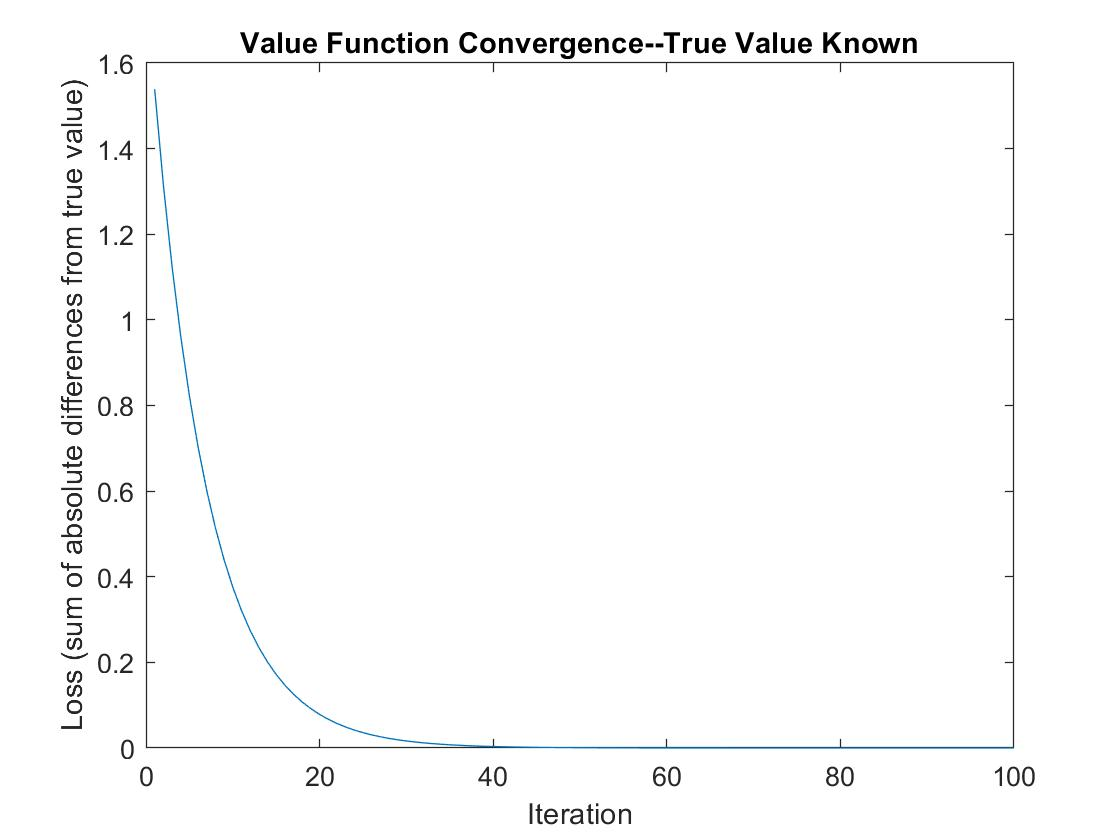
\includegraphics[width=\textwidth]{Econ_8307_PS2_4_3.jpg}
	Around 67 iterations gives a fairly precise estimate of the value function. Note 67 is the first iteration where loss function rounds to .0000.
 
	\item
	\begin{lstlisting}
 loss2 = zeros(iterations,2);
 Vold = zeros(5,1);
 Vnew = zeros(5,1);
 for i= 1:iterations
     loss2(i,1) = loss(i);
     Vold=Vnew;
     Vnew = pi + beta*(1-lambda)*T*Vold;
     for j =1:5
        loss2(i,2) = loss2(i,2) + abs(Vnew(j)-Vold(j));
     end
 end
 plot(loss2(:,1),'-')
 hold on
 plot(loss2(:,2),'--')
 title('Value Function Convergence')
 xlabel('Iteration')
 ylabel('Loss (sum of absolute differences)')
 legend({'True Value Known','True Value Unknown'},'Location','southeast')
	\end{lstlisting}
	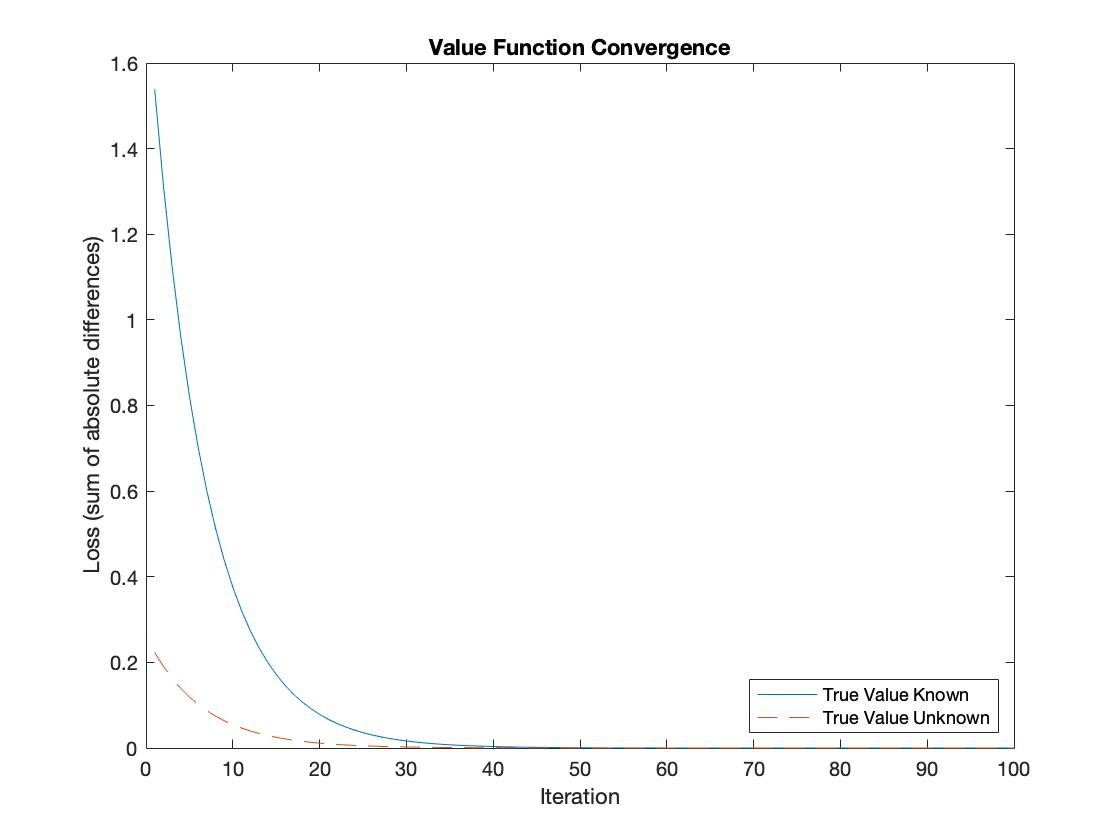
\includegraphics[width=\textwidth]{Econ_8307_PS2_4_4.jpg}
	Now around 55 iterations appears to give a fairly precise estimate of the value function. Note 55 is the first iteration where the new loss function rounds to .0000.
\end{enumerate}



\end{onehalfspace}
\end{document}
